\SetSlideHeaderLevel{section}
% ==================================================================
\section{Masalah 1: Membuat Objek yang Kaku}
% ==================================================================

\begin{frame}[t, fragile]
\frametitle{Dunia Game yang Dinamis}
\footnotesize
\begin{spacing}{0.85}
    Setelah mengelola \textit{satu} objek global (Singleton), kini kita menghadapi tantangan mengelola \textit{banyak} objek dinamis yang terus-menerus muncul dan menghilang.
\\
\medskip
\begin{columns}[T]
    \begin{column}{0.5\textwidth}
        \textbf{Definisi ``Rintangan'' (Obstacle):}
        
        Secara konseptual, rintangan adalah segala sesuatu di dalam game yang menantang pemain dan harus dihindari.
        \\
        \medskip
        Meskipun bentuknya berbeda-beda (laser, roket, dinding listrik), semuanya memiliki tujuan yang sama: menguji kemampuan pemain.
        \\
        \medskip
        \begin{alertblock}{Pertanyaan Desain}
        Bagaimana kita bisa mengelola semua jenis rintangan ini dalam satu sistem yang sama?
        \end{alertblock}
    \end{column}
    \begin{column}{0.5\textwidth}
        \centering
        \textbf{Ilustrasi Dunia Game}
        \resizebox{0.9\textwidth}{!}{
        \begin{tikzpicture}[
            player/.style={rectangle, draw, fill=blue!20, minimum size=1cm},
            obstacle/.style={rectangle, draw, rounded corners, fill=red!20},
            line/.style={draw, thick, red, ->, >=Stealth}
        ]
            \node[player] (p) at (0,0) {Player};
            \node[obstacle] (laser) at (4,1) {Laser};
            \node[obstacle] (rocket) at (4,-1) {Roket};
            
            \draw[line] (laser.west) -- (p.east);
            \draw[line] (rocket.west) -- (p.east);
            
            \node[font=\itshape, text=gray] at (4, 2) {Rintangan};
            \node[font=\itshape, text=gray] at (4, -2) {Rintangan};
        \end{tikzpicture}
        }
    \end{column}
\end{columns}
\end{spacing}
\end{frame}

\begin{frame}[t, fragile]
\frametitle{Kontrak Umum via Antarmuka}
\vspace{-2mm}
\footnotesize
\begin{spacing}{0.85}
    Untuk mengelola variasi ini, kita membuat sebuah ``kontrak'' yang harus dipatuhi semua rintangan: sebuah \textbf{antarmuka (interface)} Java.

\begin{columns}[T]
    \begin{column}{0.5\textwidth}
        \textbf{Contoh Kode Kontrak}
        
        Semua kelas rintangan \textbf{wajib} mengimplementasikan \texttt{Obstacle} dan menyediakan logika untuk metode-metodenya.
        
        \begin{minted}[fontsize=\scriptsize]{java}
// 1. Kontrak didefinisikan
public interface Obstacle {
    void update(float delta);
    void draw(SpriteBatch batch);
}
// 2. Kelas konkret mematuhinya
public class Laser implements Obstacle {
    private Vector2 position;    
    @Override
    public void update(float delta) {
        // Logika pergerakan laser...
    }
    @Override
    public void draw(SpriteBatch batch) {
        // Logika menggambar laser...
    }
}
        \end{minted}
    \end{column}
    \begin{column}{0.5\textwidth}
        \textbf{Struktur Kelas yang Diinginkan}
        
        Diagram ini memvisualisasikan kode di sebelah. \texttt{WorldController} kini bisa bekerja dengan \texttt{Obstacle} apapun secara umum.
        
        \centering
        \resizebox{\textwidth}{!}{
\begin{tikzpicture}[
    class/.style={
        rectangle, draw, fill=yellow!20, text centered, font=\small, minimum width=2.5cm, minimum height=0.8cm
    },
    interface/.style={
        rectangle split,
        rectangle split parts=3,
        draw,
        fill=green!20,
        font=\small,
        text width=4.0cm,   % agar teks terbungkus
        align=left          % supaya isi method rata kiri
    },
    impl/.style={draw, dashed, -{Triangle[open]}, shorten >=2pt},
    dep/.style={draw, dashed, -{Stealth}, shorten >=2pt}
]
    % node atas
    \node[class] (controller) at (0,3) {\textbf{WorldController}};

    % node ``interface'' dengan 3 parts:
    %  - part1: stereotype + nama
    %  - part2: (kosong atau atribut)
    %  - part3: method list (menggunakan parbox/line breaks)
    \node[interface] (obstacle) at (0,0) {
        \centering \textit{\guillemotleft interface\guillemotright}\\ \textbf{Obstacle}
        \nodepart{second}
        % jika ingin isi second, tulis di sini (saat ini kosong)
        \nodepart{third}
        \parbox[t]{\linewidth}{+ update(delta: float)\\+ draw(batch: SpriteBatch)}
    };

    % kelas turunan
    \node[class, fill=yellow!20, below left=1cm and 0.2cm of obstacle] (laser) {\textbf{Laser}};
    \node[class, fill=yellow!20, below right=1cm and 0.2cm of obstacle] (rocket) {\textbf{Rocket}};

    % hubungan
    \draw[impl] (laser) -- (obstacle);
    \draw[impl] (rocket) -- (obstacle);
    \draw[dep, thick, blue] (controller) -- (obstacle) node[midway, right, font=\tiny] {works with};
\end{tikzpicture}
        }
    \end{column}
\end{columns}
\end{spacing}
\end{frame}

\begin{frame}[t, fragile]
\frametitle{Pendekatan Naif: `\texttt{new}'}
\footnotesize
\begin{spacing}{0.85}
\begin{columns}[T]
    \begin{column}{0.5\textwidth}
        \textbf{Implementasi "Cara Buruk"}
        
        Meskipun tujuannya adalah bekerja dengan antarmuka \texttt{Obstacle}, kode ini secara langsung memanggil constructor kelas konkret.
        
        \begin{minted}[fontsize=\scriptsize]{java}
public class WorldController {
    public Obstacle createObstacle() {
        int type = new Random().nextInt(2);
        
        // Ketergantungan langsung
        // pada kelas konkret.
        // Ini adalah "code smell".
        if (type == 0) {
            return new Laser();
        } else {
            return new Rocket();
        }
    }
}
        \end{minted}
    \end{column}
    \begin{column}{0.5\textwidth}
        \textbf{Masalah yang Timbul}
        
        Pendekatan ini secara langsung menciptakan ketergantungan yang kaku.
        \begin{itemize}
            \item \texttt{WorldController} sekarang harus tahu tentang setiap jenis rintangan yang ada.
            \item Setiap kali ada rintangan baru (misal: \texttt{Missile}), kita \textbf{wajib} memodifikasi file \texttt{WorldController}.
            \item Ini membuat kode kita rapuh dan sulit untuk dikembangkan.
        \end{itemize}
        
        \begin{alertblock}{Problem Utama}
        Pendekatan ini melanggar \textbf{Prinsip Open/Closed}, salah satu pilar desain perangkat lunak yang baik.
        \end{alertblock}
    \end{column}
\end{columns}
\end{spacing}
\end{frame}

\subsection{Konsekuensi}
\SetSlideHeaderLevel{subsection}

\begin{frame}[t, fragile]
\frametitle{1: Risiko Bug Baru}
\footnotesize
\begin{spacing}{0.85}
    Setiap kali kita memodifikasi file yang sudah stabil dan berfungsi, kita membuka pintu bagi bug-bug baru yang tidak disengaja.

    \begin{columns}[T]
        \begin{column}{0.5\textwidth}
            \textbf{Penjelasan Risiko}
            
            \texttt{WorldController} adalah kelas inti yang sangat penting. Mengubahnya untuk menambah rintangan \texttt{Missile} bisa saja secara tidak sengaja merusak fungsionalitas yang sudah ada.
            
            \begin{itemize}
                \item Kesalahan copy-paste.
                \item Lupa menambahkan `break' dalam `switch'.
                \item Mengubah logika random yang sudah ada.
                \item dan lain-lain.
            \end{itemize}
            
            Perubahan sekecil apa pun memiliki risiko. Prinsip Open/Closed bertujuan untuk meminimalkan risiko ini.
            
        \end{column}
        \begin{column}{0.5\textwidth}
            \textbf{Contoh Bug Akibat Modifikasi}
            
            Saat menambahkan \texttt{Missile}, terjadi kesalahan copy-paste yang fatal: kasus 3 malah membuat \texttt{Rocket}.
            
            \begin{minted}[fontsize=\scriptsize, bgcolor=softred]{java}
public class WorldController {
    public Obstacle createObstacle() {
        int type = new Random().nextInt(4);
        switch (type) {
            case 0: return new Laser();
            case 1: return new Rocket();
            case 2: return new Zapper();
            case 3: 
                // BUG! Seharusnya 'new Missile()'
                // malah membuat Rocket lagi.
                return new Rocket(); 
        }
        return null;
    }
}
            \end{minted}
        \end{column}
    \end{columns}
\end{spacing}
\end{frame}

\begin{frame}[t, fragile]
\frametitle{2: Testing yang Berulang}
\footnotesize
\vspace{-2mm}
\begin{spacing}{0.8}
    Karena file inti diubah, kita tidak bisa hanya menguji fitur baru, melainkan juga semua fungsionalitas lama untuk memastikan tidak ada yang rusak.

    \begin{columns}[T]
        \begin{column}{0.45\textwidth}
            \textbf{Penjelasan Masalah}
            
            Proses pengujian menjadi tidak efisien. Setiap kali rintangan baru ditambahkan:
            \begin{itemize}
                \item \textbf{Pengujian Fitur Baru:} Anda harus membuat tes untuk memastikan rintangan baru (misal: `Missile') berfungsi.
                \item \textbf{Pengujian Regresi:} Anda juga \textbf{wajib} menjalankan kembali semua tes lama untuk `Laser', `Rocket', dan `Zapper' untuk memastikan modifikasi Anda tidak merusak mereka.
            \end{itemize}
            
            Ini membuang-buang waktu dan sumber daya, terutama pada proyek besar.
            
        \end{column}
        \begin{column}{0.55\textwidth}
        \vspace{-3mm}
            \textbf{Contoh Kode Uji (Illustrasi)}
            
            Perubahan pada \texttt{WorldController} memaksa kita menjalankan kembali tes-tes lama.
            
            \begin{minted}[fontsize=\scriptsize, bgcolor=gray!10]{java}
// WorldControllerTest.java
// Tes untuk fitur baru
@Test
void testSpawnMissile() {
    // ...
}
/**
 * Karena WorldController.java dimodifikasi,
 * semua tes ini WAJIB dijalankan kembali
 * untuk mencegah regresi (kerusakan fitur lama).
 */
@Test
void testSpawnLaser_Regression() {
    // ...
}
@Test
void testSpawnRocket_Regression() {
    // ...
}
            \end{minted}
        \end{column}
    \end{columns}
\end{spacing}
\end{frame}

\begin{frame}[t, fragile]
\frametitle{3: Bottleneck Kolaborasi Tim}
\footnotesize
\begin{spacing}{0.85}
    Dalam lingkungan tim, jika semua orang harus mengubah file pusat yang sama, ini akan menciptakan ``kemacetan'' dan memperlambat pengembangan.

    \begin{columns}[T]
        \begin{column}{0.5\textwidth}
            \textbf{Penjelasan Masalah}
            
            Bayangkan sebuah tim dengan dua developer:
            \begin{itemize}
                \item \textbf{Developer A} ditugaskan membuat rintangan \texttt{Shield}.
                \item \textbf{Developer B} ditugaskan membuat rintangan \texttt{Mine}.
            \end{itemize}
            
            Keduanya akan mengubah file yang sama, yaitu \texttt{WorldController.java}. Saat mereka mencoba menggabungkan pekerjaan mereka, akan terjadi \textbf{merge conflict}—sebuah situasi di mana sistem kontrol versi (seperti Git) tidak tahu bagaimana cara menggabungkan kedua perubahan tersebut secara otomatis.
            
        \end{column}
        \begin{column}{0.5\textwidth}
            \textbf{Contoh Merge Conflict di Git}
            
            Sistem akan menandai area konflik yang harus diselesaikan secara manual.
            
            \begin{minted}[fontsize=\scriptsize, bgcolor=softred]{diff}
// File: WorldController.java

    case 2: return new Zapper();
<<<<<<< HEAD (Perubahan Anda)
    case 3: return new Shield();
=======
    case 3: return new Mine();
>>>>>>> branch-developer-B
}
            \end{minted}
            
            \begin{alertblock}{Dampak}
            Menyelesaikan konflik seperti ini membuang waktu, berisiko menimbulkan bug, dan menjadi \textit{bottleneck} yang menghambat produktivitas tim.
            \end{alertblock}
            
        \end{column}
    \end{columns}
\end{spacing}
\end{frame}

\begin{frame}[t, fragile]
\frametitle{Struktur \& Implementasi yang Buruk}
\footnotesize
\vspace{-2mm}
\begin{spacing}{0.85}
\begin{columns}[T]
    \begin{column}{0.5\textwidth}
        \textbf{Struktur Ketergantungan yang Kaku}
        
        Diagram kelas menunjukkan bagaimana \texttt{WorldController} menjadi terikat erat (tightly coupled) dengan setiap kelas rintangan konkret.
        
        \centering
        \resizebox{\textwidth}{!}{
        \begin{tikzpicture}[
            class/.style={rectangle, draw, fill=yellow!20, text width=3cm, text centered},
            dep/.style={draw, dashed, ->, >=Stealth}
        ]
            \node[class] (controller) at (0,2) {\textbf{WorldController}};
            \node[class] (laser) at (-2,0) {\textbf{Laser}};
            \node[class] (rocket) at (2,0) {\textbf{Rocket}};
            
            \draw[dep, thick, red] (controller) -- (laser) node[midway, above, sloped, font=\tiny]{creates};
            \draw[dep, thick, red] (controller) -- (rocket) node[midway, above, sloped, font=\tiny]{creates};
        \end{tikzpicture}
        }
    \end{column}
    \begin{column}{0.5\textwidth}
        \textbf{Melanggar Prinsip Open/Closed}
        
        Prinsip ini menyatakan: ``Sebuah kelas harus terbuka untuk \textbf{ekstensi} (menambah rintangan baru), tetapi tertutup untuk \textbf{modifikasi}.''
        
        \begin{minted}[fontsize=\scriptsize, bgcolor=softred]{java}
// Untuk menambah Missile, kita WAJIB
// memodifikasi file ini.
public class WorldController {
    public Obstacle createObstacle() {
        int type = new Random().nextInt(3);
        switch (type) {
            case 0: return new Laser();
            case 1: return new Rocket();
            // MODIFIKASI DIMULAI DI SINI
            case 2: return new Missile(); 
        }
        return null;
    }
}
        \end{minted}
    \end{column}
\end{columns}

\begin{alertblock}{Justifikasi Kebutuhan Pola Desain}
Kita butuh cara untuk mendelegasikan proses pembuatan objek, sehingga \texttt{WorldController} tidak perlu tahu tentang kelas-kelas rintangan yang spesifik.
\end{alertblock}
\end{spacing}
\end{frame}

% ==================================================================
\subsection{Solusi: Factory Method}
% ==================================================================

\begin{frame}[t, fragile]
\frametitle{The Factory Method Pattern}
\footnotesize
\begin{spacing}{0.85}
    \begin{beamercolorbox}[rounded=true,shadow=true]{block title}
        \centering
        \textbf{Intent: Mendefinisikan antarmuka untuk membuat objek, namun membiarkan subclass yang memutuskan kelas mana yang akan diinstansiasi.}
    \end{beamercolorbox}

    \vspace{0.5cm}
    \textbf{Analogi: Pabrik Kendaraan}
    \begin{itemize}
        \item Ada sebuah cetak biru \texttt{Pabrik} abstrak yang memiliki metode \texttt{buatKendaraan()}.
        \item \texttt{PabrikMobil} (subclass) mengimplementasikan metode itu untuk menghasilkan \texttt{new Mobil()}.
        \item \texttt{PabrikMotor} (subclass) mengimplementasikan metode itu untuk menghasilkan \texttt{new Motor()}.
    \end{itemize}
    \vspace{0.5cm}
    Logika utama kita hanya perlu berinteraksi dengan \texttt{Pabrik} abstrak, tanpa perlu tahu produk konkret apa yang dibuatnya.
\end{spacing}
\end{frame}

\begin{frame}[t, fragile]
\frametitle{Class Diagram}
\footnotesize
\begin{spacing}{0.85}
\begin{columns}[T]
    \begin{column}{0.6\textwidth}
    \centering
    \resizebox{\textwidth}{!}{
    \begin{tikzpicture}[
        node distance=1.5cm and 3.5cm, % Jarak horizontal direnggangkan
        class/.style={rectangle, draw, fill=yellow!20, font=\small, minimum width=3.5cm, text centered},
        absclass/.style={rectangle split, rectangle split parts=3, draw, fill=yellow!30, font=\small, text width=4cm, align=left},
        interface/.style={rectangle split, rectangle split parts=3, draw, fill=green!20, font=\small, text width=4cm, align=left},
        impl/.style={draw, dashed, -{Triangle[open]}, shorten >=2pt},
        dep/.style={draw, dashed, -{Stealth}, shorten >=2pt}
    ]
        % Creators
        \node[absclass] (creator) at (0,0) {
            \centering\textit{\guillemotleft abstract class\guillemotright}\\\textbf{ObstacleFactory}
            \nodepart{second}
            \nodepart{third}
            \textit{+ createObstacle(): Obstacle}
        };
        \node[class, below left=1cm and 0.1cm of creator] (laserFactory) {\textbf{LaserFactory}};
        \node[class, below right=1cm and 0.1cm of creator] (rocketFactory) {\textbf{RocketFactory}};
        
        % Products
        \node[interface] (product) at (0,-5) { % Posisi digeser ke kanan
            \centering\textit{\guillemotleft interface\guillemotright}\\\textbf{Obstacle}
            \nodepart{second}
            \nodepart{third}
            + update() \\ + draw()
        };
        \node[class, below left=1cm and 0.1cm of product] (laser) {\textbf{Laser}};
        \node[class, below right=1cm and 0.1cm of product] (rocket) {\textbf{Rocket}};
        
        % Relationships
        \draw[impl] (laserFactory) -- (creator);
        \draw[impl] (rocketFactory) -- (creator);
        \draw[impl] (laser) -- (product);
        \draw[impl] (rocket) -- (product);
        
        \draw[dep] (laserFactory) -- (laser) node[midway, below, sloped, font=\tiny]{creates};
        \draw[dep] (rocketFactory) -- (rocket) node[midway, below, sloped, font=\tiny]{creates};
        \draw[dep] (creator) -- (product) node[midway, above, font=\tiny]{returns};
    \end{tikzpicture}
    }
    \end{column}
    \begin{column}{0.4\textwidth}
    \begin{block}{Struktur Pola}
    \begin{itemize}
        \item \textbf{Creator Abstrak (\texttt{ObstacleFactory}):} Mendefinisikan ``kontrak'' atau metode pabrik.
        \item \textbf{Concrete Creator (\texttt{LaserFactory}, dll):} Mengimplementasikan metode pabrik untuk membuat produk konkret.
        \item \textbf{Product (\texttt{Obstacle}):} Antarmuka umum untuk semua produk yang bisa dibuat.
    \end{itemize}
    \end{block}
    \end{column}
\end{columns}
\end{spacing}
\end{frame}

\begin{frame}[t, fragile]
\frametitle{Sebelum vs. Sesudah Factory Method}
\footnotesize
\begin{spacing}{0.85}
\begin{columns}[T]
    \begin{column}{0.5\textwidth}
        \textbf{Sebelum: Terikat Erat}
        \begin{minted}[fontsize=\scriptsize, bgcolor=softred]{java}
public class WorldController {
    public void spawnObstacle() {
        Obstacle obs = null;
        int type = ...;
        // Logika pembuatan ada di sini
        switch (type) {
            case 0: obs = new Laser();
                    break;
            case 1: obs = new Rocket();
                    break;
        }
        // ...
    }
}
        \end{minted}
    \end{column}
    \begin{column}{0.5\textwidth}
        \textbf{Sesudah: Fleksibel \& Terpisah}
        \begin{minted}[fontsize=\scriptsize, bgcolor=softgreen]{java}
// Factory didefinisikan di tempat lain
ObstacleFactory factory = new LaserFactory();
// ... atau new RocketFactory();

public class WorldController {
    public void spawnObstacle(
                ObstacleFactory factory) {
        // Delegasikan pembuatan objek!
        Obstacle obs = factory.createObstacle();
        // ...
    }
}
        \end{minted}
    \end{column}
\end{columns}

\begin{alertblock}{Keuntungan Langsung}
\texttt{WorldController} kini tidak tahu menahu tentang \texttt{Laser} atau \texttt{Rocket}. Untuk menambah \texttt{Missile}, kita hanya perlu membuat \texttt{MissileFactory} baru tanpa menyentuh \texttt{WorldController} sama sekali. Prinsip Open/Closed terpenuhi!
\end{alertblock}
\end{spacing}
\end{frame}

\begin{frame}[t, fragile]
\frametitle{Melihat ke Dalam Pabrik}
\footnotesize
\vspace{-2mm}
\begin{spacing}{0.8}
    Slide sebelumnya menunjukkan \texttt{WorldController} yang ``bersih''. Kebersihan itu tercapai dengan memindahkan logika pembuatan objek ke dalam kelas-kelas Factory.

    \begin{columns}[T]
        \begin{column}{0.5\textwidth}
            \textbf{1. Kontrak (Creator Abstrak)}
            
            Kelas abstrak ini mendefinisikan metode \texttt{createObstacle()} yang wajib diimplementasikan oleh semua pabrik konkret.
            
            \begin{minted}[fontsize=\scriptsize, bgcolor=yellow!10]{java}
public abstract class ObstacleFactory { 
    /**
     * The Factory Method.
     * Subclass akan override metode ini
     * untuk membuat produk spesifik.
     */
    public abstract Obstacle createObstacle();

    // Creator juga bisa punya logika lain
    public void someBaseOperation() {
        // ...
    }
}
            \end{minted}
        \end{column}
        \begin{column}{0.5\textwidth}
        \vspace{-3mm}
            \textbf{2. Implementasi (Concrete Creators)}
            
            Setiap pabrik konkret hanya punya satu tanggung jawab: membuat satu jenis objek.
            
            \begin{minted}[fontsize=\scriptsize, bgcolor=green!5]{java}
public class LaserFactory extends ObstacleFactory {
    @Override
    public Obstacle createObstacle() {
        // Di sinilah 'new Laser()' berada
        return new Laser();
    }
}
public class RocketFactory extends ObstacleFactory {
    @Override
    public Obstacle createObstacle() {
        // Di sinilah 'new Rocket()' berada
        return new Rocket();
    }
}
            \end{minted}
        \end{column}
    \end{columns}
    \vspace{-3mm}
    \begin{alertblock}{Pemisahan Tanggung Jawab}
    Operator \texttt{new} yang tadinya ``mengotori'' logika utama \texttt{WorldController} kini telah dienkapsulasi dengan rapi di dalam kelas-kelas Factory yang sesuai.
    \end{alertblock}

\end{spacing}
\end{frame}

% ==================================================================
\subsection{Keunggulan Factory Method}
% ==================================================================

\begin{frame}[t, fragile]
\frametitle{1: Menghindari Bug Baru}
\footnotesize
\vspace{-2mm}
\begin{spacing}{0.8}
    Mari kita lihat bagaimana Factory Method menanggulangi tiga konsekuensi buruk yang telah kita bahas.
\vspace{-0.5mm}
    \begin{columns}[T]
        \begin{column}{0.5\textwidth}
            \textbf{Penjelasan Solusi}
            
            Dengan Factory Method, \texttt{WorldController.java} \textbf{tidak pernah dimodifikasi}. Untuk menambah rintangan \texttt{Missile}, kita hanya perlu \textbf{membuat file baru} yang terisolasi.
            
            \begin{itemize}
                \item Risiko merusak logika inti di \texttt{WorldController} menjadi nol, karena file tersebut tidak disentuh.
                \item Pekerjaan kita terfokus pada pembuatan kelas baru (\texttt{Missile} dan \texttt{MissileFactory}), yang lebih aman.
            \end{itemize}
            
            Ini adalah perwujudan nyata dari Prinsip Open/Closed: kelas inti \textbf{tertutup} untuk modifikasi, namun sistem tetap \textbf{terbuka} untuk ekstensi.
        \end{column}
        \begin{column}{0.5\textwidth}
            \textbf{Contoh Penambahan Fitur yang Aman}
            
            Untuk menambah rintangan \texttt{Missile}, kita membuat:
            
            \begin{minted}[fontsize=\scriptsize, bgcolor=softgreen]{java}
// File Baru 1: Missile.java
public class Missile implements Obstacle {
    // ...
}
// File Baru 2: MissileFactory.java
public class MissileFactory extends ObstacleFactory {
    @Override
    public Obstacle createObstacle() {
        return new Missile();
    }
}
            \end{minted}
            \begin{minted}[fontsize=\scriptsize, bgcolor=gray!10]{java}
// File WorldController.java TIDAK BERUBAH!
public class WorldController {
    public void spawnObstacle(
                ObstacleFactory factory) {
        Obstacle obs = factory.createObstacle();
        // ...
    }
}
            \end{minted}
        \end{column}
    \end{columns}
\end{spacing}
\end{frame}

\begin{frame}[t, fragile]
\frametitle{2: Testing yang Efisien}
\footnotesize
\begin{spacing}{0.85}
    Karena kode inti tidak berubah, proses pengujian menjadi jauh lebih efisien dan terfokus.

    \begin{columns}[T]
        \begin{column}{0.5\textwidth}
            \textbf{Penjelasan Solusi}
            
            Setelah menambah rintangan \texttt{Missile}:
            \begin{itemize}
                \item Kita \textbf{tidak perlu} menjalankan tes regresi untuk \texttt{WorldController}, karena kodenya tidak berubah. Kita percaya fungsionalitasnya masih stabil.
                \item Kita hanya perlu membuat \textbf{satu set tes baru} yang spesifik untuk \texttt{MissileFactory}.
            \end{itemize}
            
            Ini menghemat waktu secara signifikan dan membuat proses pengujian menjadi lebih logis. Kita hanya menguji apa yang baru atau yang berubah.
            
        \end{column}
        \begin{column}{0.5\textwidth}
            \textbf{Contoh Kode Uji yang Terfokus}
            
            Alih-alih menguji ulang \texttt{WorldController}, kita membuat file tes baru yang terisolasi.
            
            \begin{minted}[fontsize=\scriptsize, bgcolor=softgreen]{java}
// File Baru: MissileFactoryTest.java
public class MissileFactoryTest {
    @Test
    void factoryCreatesCorrectTypeOfObstacle() {
        // Arrange
        ObstacleFactory factory = new MissileFactory();        
        // Act
        Obstacle created = factory.createObstacle();       
        // Assert
        // Pastikan pabrik membuat objek yang benar
        assertTrue(created instanceof Missile);
    }
}
            \end{minted}
        \end{column}
    \end{columns}
\end{spacing}
\end{frame}

\begin{frame}[t, fragile]
\frametitle{3: Kolaborasi yang Lancar}
\footnotesize
\begin{spacing}{0.85}
    Masalah \textit{merge conflict} pada file pusat dapat dihindari sepenuhnya, memungkinkan tim untuk bekerja secara paralel tanpa hambatan.

    \begin{columns}[T]
        \begin{column}{0.5\textwidth}
            \textbf{Penjelasan Solusi}
            
            Kembali ke skenario dua developer:
            \begin{itemize}
                \item \textbf{Developer A} sekarang bekerja pada file-file baru: \texttt{Shield.java} dan \texttt{ShieldFactory.java}.
                \item \textbf{Developer B} bekerja pada file-file baru yang berbeda: \texttt{Mine.java} dan \texttt{MineFactory.java}.
            \end{itemize}
            
            Karena mereka bekerja pada file yang sepenuhnya terpisah, tidak akan ada \textit{merge conflict}. Mereka bisa menggabungkan pekerjaan mereka dengan aman dan cepat.
            
        \end{column}
        \begin{column}{0.5\textwidth}
            \textbf{Contoh Struktur File Paralel}
            
            Setiap developer bekerja di ``wilayah'' mereka sendiri tanpa mengganggu orang lain.
            
            \begin{minted}[fontsize=\scriptsize, bgcolor=softgreen]{text}
src/
 |- obstacles/
 |   |- Shield.java       (Milik Dev A)
 |   '- Mine.java         (Milik Dev B)
 |
 |- factories/
 |   |- ShieldFactory.java  (Milik Dev A)
 |   '- MineFactory.java    (Milik Dev B)
 |
 '- controllers/
     '- WorldController.java (Tidak diubah)
            \end{minted}
            
            \begin{alertblock}{Hasil}
            Pengembangan menjadi lebih cepat, lebih aman, dan lebih mudah untuk diskalakan seiring bertambahnya anggota tim dan fitur.
            \end{alertblock}
            
        \end{column}
    \end{columns}
\end{spacing}
\end{frame}

\subsection{Kelemahan Factory Method}
\begin{frame}[t, fragile]
\frametitle{Proliferasi Kelas}
\footnotesize
\begin{spacing}{0.85}
    Tidak ada solusi yang sempurna. Factory Method memecahkan masalah modifikasi, namun memperkenalkan \textit{trade-off} baru: jumlah kelas yang membengkak.

    \begin{columns}[T]
        \begin{column}{0.5\textwidth}
            \textbf{Penjelasan Masalah}
            
            Pola ini sangat patuh pada Prinsip Open/Closed, tetapi akibatnya adalah setiap kali kita ingin menambah \textbf{satu} jenis rintangan baru, kita harus membuat \textbf{dua} file kelas baru:
            \begin{itemize}
                \item Kelas produk itu sendiri (misal: \texttt{Missile.java}).
                \item Kelas pabrik untuk produk tersebut (misal: \texttt{MissileFactory.java}).
            \end{itemize}
            
            Untuk game dengan puluhan atau ratusan jenis objek, ini bisa menyebabkan "ledakan kelas" yang membuat manajemen proyek menjadi lebih rumit.
            
        \begin{alertblock}{Trade-off}
        Kita menukar risiko modifikasi file inti dengan kompleksitas manajemen jumlah file yang lebih banyak.
        \end{alertblock}
        \end{column}
        \begin{column}{0.5\textwidth}
            \textbf{Contoh "Ledakan Kelas"}
            
            Struktur direktori bisa menjadi sangat padat dengan cepat.
            
            \begin{minted}[fontsize=\scriptsize, bgcolor=gray!10]{text}
src/
 |- obstacles/
 |   |- Laser.java
 |   |- Rocket.java
 |   |- Missile.java
 |   |- Shield.java
 |   |- Mine.java
 |   '- ... (puluhan file lagi)
 |
 '- factories/
     |- LaserFactory.java
     |- RocketFactory.java
     |- MissileFactory.java
     |- ShieldFactory.java
     |- MineFactory.java
     '- ... (puluhan file lagi)
            \end{minted}
            
        \end{column}
    \end{columns}            
\end{spacing}
\end{frame}

\begin{frame}[t, fragile]
\frametitle{Masalah yang Belum Terselesaikan}
\footnotesize
\begin{spacing}{0.85}
    Factory Method telah berhasil memecahkan masalah \textbf{fleksibilitas} desain. Namun, ia sama sekali tidak menyentuh masalah krusial lain dalam game development: \textbf{performa}.

    \begin{columns}[T]
        \begin{column}{0.5\textwidth}
            \textbf{Akar Masalah Performa}
            
            Meskipun kita sudah mendelegasikan pembuatan objek, setiap panggilan ke \texttt{factory.createObstacle()} pada akhirnya tetap berujung pada satu hal:
            
            \begin{itemize}
                \item Eksekusi operator \textbf{\texttt{new}}.
            \end{itemize}
            
            Di dalam game yang memunculkan ratusan peluru atau koin per detik, memanggil \texttt{new} secara terus-menerus akan menjadi \textit{bottleneck} performa yang signifikan dan membebani Garbage Collector.
            
            \begin{alertblock}{Pertanyaan Berikutnya}
            Bagaimana jika kita bisa mendapatkan objek tanpa harus selalu memanggil \texttt{new}?
            \end{alertblock}
            
        \end{column}
        \begin{column}{0.5\textwidth}
            \textbf{Operator `new' Tetap Ada}
            
            Di balik semua abstraksi, panggilan \texttt{new} yang ``mahal'' masih menjadi inti dari setiap pabrik.
            
            \begin{minted}[fontsize=\scriptsize, bgcolor=softred]{java}
// Di dalam MissileFactory.java

@Override
public Obstacle createObstacle() {
    /**
     * Masalah fleksibilitas teratasi,
     * tetapi masalah performa akibat
     * 'new' masih ada di sini.
     */
    return new Missile();
}
            \end{minted}
        \end{column}
    \end{columns}
\end{spacing}
\end{frame}

% ==================================================================
\section{Masalah 2: Performa \& Alokasi Memori}
% ==================================================================
\SetSlideHeaderLevel{section}
\begin{frame}[t, fragile]
\frametitle{Frekuensi Pembuatan Objek}
\vspace{-2mm}
\footnotesize
\begin{spacing}{0.8}
    Factory Method menyelesaikan masalah \textit{fleksibilitas}, tapi tidak \textit{efisiensi}. Dalam game, masalah efisiensi muncul dari skala: kita membuat \textbf{sangat banyak} objek dalam waktu singkat.
    \\
    \medskip
    
        \textbf{Skenario Game Penuh Aksi}
        
        Bayangkan sebuah game \textit{bullet hell} atau \textit{endless runner}:
        \begin{itemize}
            \item Pemain menembakkan puluhan peluru per detik.
            \item Ratusan koin muncul di layar.
            \item Efek partikel ledakan tercipta dan menghilang.
        \end{itemize}
        
        Setiap objek ini, sekecil apa pun, biasanya dibuat dengan panggilan \texttt{new}. Ini seperti menembakkan senapan mesin yang pelurunya adalah permintaan alokasi memori.
        \\
        \medskip
        
        \textbf{Ilustrasi: ``Hujan'' Panggilan \texttt{new}}
        
        Dalam satu detik, game loop bisa memanggil \texttt{new} ratusan kali.
        \\
        \medskip
        
        \centering
        \resizebox{\textwidth}{!}{
        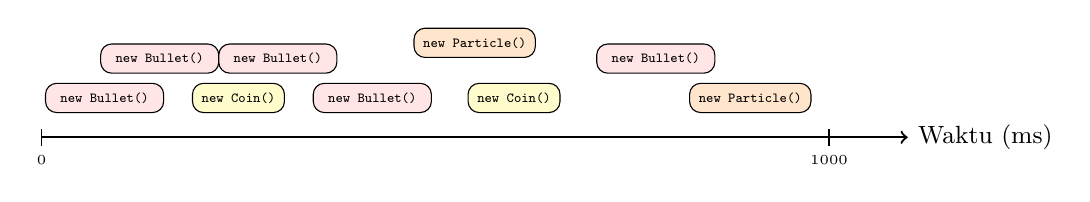
\begin{tikzpicture}[font=\tiny]
            \draw[->, thick] (0,0) -- (11,0) node[right, font=\small] {Waktu (ms)};
            \draw (0, 3pt) -- (0, -3pt) node[below] {0};
            \draw (10, 3pt) -- (10, -3pt) node[below] {1000};
            
            \node[draw, fill=red!10, rounded corners, minimum width=1.5cm] at (0.8, 0.5) {\texttt{new Bullet()}};
            \node[draw, fill=red!10, rounded corners, minimum width=1.5cm] at (1.5, 1.0) {\texttt{new Bullet()}};
            \node[draw, fill=yellow!20, rounded corners] at (2.5, 0.5) {\texttt{new Coin()}};
            \node[draw, fill=red!10, rounded corners, minimum width=1.5cm] at (3.0, 1.0) {\texttt{new Bullet()}};
            \node[draw, fill=red!10, rounded corners, minimum width=1.5cm] at (4.2, 0.5) {\texttt{new Bullet()}};
            \node[draw, fill=orange!20, rounded corners] at (5.5, 1.2) {\texttt{new Particle()}};
            \node[draw, fill=yellow!20, rounded corners] at (6.0, 0.5) {\texttt{new Coin()}};
            \node[draw, fill=red!10, rounded corners, minimum width=1.5cm] at (7.8, 1.0) {\texttt{new Bullet()}};
            \node[draw, fill=orange!20, rounded corners] at (9.0, 0.5) {\texttt{new Particle()}};
        \end{tikzpicture}
        }
\end{spacing}
\end{frame}

\subsection{Konsekuensi}
\SetSlideHeaderLevel{subsection}

\begin{frame}[t, fragile]
\frametitle{Anatomi Biaya: Proses Alokasi Memori}
\footnotesize
\begin{spacing}{0.85}
    Mengapa memanggil \texttt{new} secara berlebihan itu ``mahal''? Karena ini memicu proses alokasi memori di area yang disebut \textbf{Heap}.

    \begin{columns}[T]
        \begin{column}{0.5\textwidth}
            \textbf{Proses di Balik Operator \texttt{new}:}
            \begin{enumerate}
                \item \textbf{Permintaan Alokasi:} Aplikasi meminta ke JVM: "Saya butuh blok memori sebesar X byte untuk objek \texttt{Bullet}."
                \item \textbf{Pencarian Blok Kosong:} JVM harus memindai Heap untuk mencari area kosong yang cukup besar. Proses ini tidak instan.
                \item \textbf{Inisialisasi \& Konstruksi:} Setelah blok ditemukan, memori diinisialisasi dan constructor objek dijalankan.
                \item \textbf{Meninggalkan ``Sampah'':} Ketika peluru menghilang dari layar, objeknya menjadi tidak terpakai (sampah), tetapi memorinya tidak langsung kembali.
            \end{enumerate}
            
        \end{column}
        \begin{column}{0.5\textwidth}
            \textbf{Ilustrasi Sederhana Heap Memori}
            
            \centering
            \resizebox{\textwidth}{!}{
            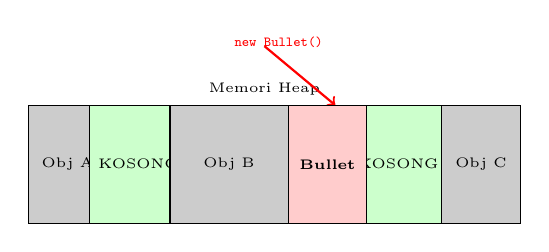
\begin{tikzpicture}[
                font=\tiny,
                heap/.style={rectangle, draw, minimum width=6cm, minimum height=1.5cm, label=above:Memori Heap},
                used/.style={rectangle, draw, fill=gray!40, minimum height=1.5cm},
                free/.style={rectangle, draw, fill=green!20, minimum height=1.5cm},
                new/.style={rectangle, draw, fill=red!20, minimum height=1.5cm}
            ]
                \node[heap] (heap) {};
                \node[used, minimum width=1cm] at (-2.5, 0) {Obj A};
                \node[free, minimum width=0.8cm] at (-1.6, 0) {KOSONG};
                \node[used, minimum width=1.5cm] at (-0.45, 0) {Obj B};
                \node[free, minimum width=1.25cm] at (1.7, 0) {KOSONG};
                \node[used, minimum width=1.0cm] at (2.75, 0) {Obj C};
                
                \draw[->, thick, red] (0, 1.5) -- (0.9, 0.75) node[above, pos=0.2] {\texttt{new Bullet()}};
                \node[new, minimum width=1cm] at (0.8, 0) {\textbf{Bullet}};
            \end{tikzpicture}
            }
            \small\textit{JVM harus mencari celah ``KOSONG'' yang pas.}
        \end{column}
    \end{columns}
\end{spacing}
\end{frame}

\begin{frame}[t, fragile]
\frametitle{Jeda Akibat Garbage Collection (GC)}
\footnotesize
\vspace{-2mm}
\begin{spacing}{0.8}
    ``Sampah'' memori yang menumpuk harus dibersihkan. Tugas ini dilakukan oleh proses otomatis bernama \textbf{Garbage Collector (GC)}.
    \\
    \medskip
    
            \textbf{Masalah Utama GC dalam Game}
            
            GC adalah fitur luar biasa, tapi punya satu kelemahan fatal untuk aplikasi real-time:
            \begin{itemize}
                \item Untuk bisa bekerja dengan aman, GC seringkali harus \textbf{menghentikan total} eksekusi aplikasi Anda selama beberapa milidetik. Ini disebut jeda \textbf{``Stop-the-World''}.
                \item Di dunia web, jeda 50ms mungkin tidak terasa.
                \item Di dunia game yang berjalan 60 frame per detik (16ms per frame), jeda 50ms berarti Anda kehilangan \textbf{tiga frame penuh}.
            \end{itemize}
            
            \begin{alertblock}{Hasil Akhir}
            Jeda ini dirasakan oleh pemain sebagai \textit{stutter}, \textit{hiccup}, atau \textit{lag} yang sangat mengganggu.
            \end{alertblock}
            
            \centering
            \resizebox{0.8\textwidth}{!}{
            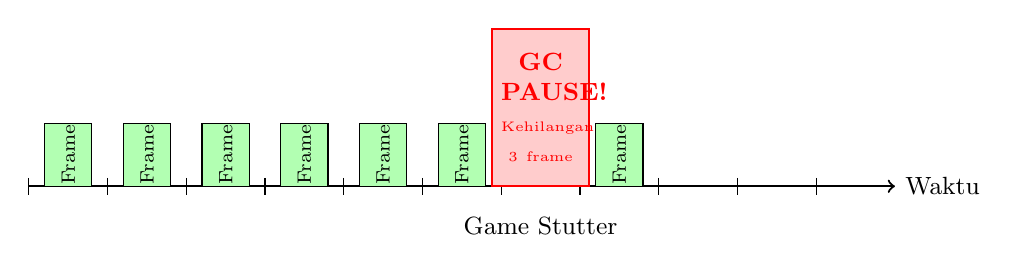
\begin{tikzpicture}[font=\small]
                \draw[->, thick] (0,0) -- (11,0) node[right] {Waktu};
                \foreach \x in {0,1,...,10} \draw (\x, 3pt) -- (\x, -3pt);

                \foreach \x in {0.5, 1.5, ..., 5.5, 7.5, ..., 9.5}
                    \draw[fill=green!30] (\x-0.3, 0.0) rectangle (\x+0.3, 0.8) node[midway, rotate=90] {\scriptsize Frame};
                
                \node[draw, red, thick, fill=red!20, minimum height=2cm,
                      minimum width=1.2cm, text width=1cm, align=center]
                      at (6.5, 1) {\textbf{GC PAUSE!}\\ \tiny Kehilangan 3 frame};
                \node at (6.5, -0.5) {Game Stutter};
            \end{tikzpicture}
            }
\end{spacing}
\end{frame}

% ==================================================================
\subsection{Solusi: Object Pool}
% ==================================================================

\begin{frame}[t, fragile]
\frametitle{The Object Pool Pattern}
\footnotesize
\begin{spacing}{0.85}
    \begin{beamercolorbox}[rounded=true,shadow=true]{block title}
        \centering
        \textbf{Intent: Meningkatkan performa secara signifikan dengan mendaur ulang objek yang tidak lagi digunakan, daripada membuat instance baru.}
    \end{beamercolorbox}

    \vspace{0.5cm}
    \textbf{Analogi: Perpustakaan Buku}
    \begin{itemize}
        \item Alih-alih \textbf{membeli buku baru} setiap kali ingin membaca (\texttt{new}), Anda pergi ke \textbf{perpustakaan} (Object Pool).
        \item Anda \textbf{meminjam} buku yang tersedia (\texttt{acquire()}).
        \item Setelah selesai, Anda \textbf{mengembalikannya} (\texttt{release()}) agar bisa dipinjam orang lain.
    \end{itemize}
    \vspace{0.5cm}
    Ini menghindari pemborosan (alokasi memori) dan mengurangi ``sampah'' (objek yang perlu di-GC).
\end{spacing}
\end{frame}

\begin{frame}[t, fragile]
\frametitle{Alur Kerja (1/2): Peminjaman Objek}
\footnotesize
\begin{spacing}{0.85}
\begin{columns}[T]
    \begin{column}{0.6\textwidth}
        \centering
        \resizebox{\textwidth}{!}{
        % --- KODE YANG TELAH DIPERBAIKI ---
        \begin{tikzpicture}[
            node distance=1.5cm and 3cm,
            lifeline/.style={draw, thick},
            object/.style={rectangle, draw, rounded corners, fill=blue!10, text centered, minimum width=2.5cm, minimum height=0.8cm},
            msg/.style={draw, -{Stealth[length=2.5mm]}},
            ret_msg/.style={draw, dashed, -{Stealth[length=2.5mm]}}
        ]
            % Objek
            \node[object] (client) {\footnotesize :Client};
            \node[object, right=of client] (pool) {\footnotesize :BulletPool};
            \node[object, right=of pool] (bullet) {\footnotesize b:Bullet};
            
            % Lifelines
            \draw[lifeline] (client.south) -- ++(0,-5);
            \draw[lifeline] (pool.south) -- ++(0,-5);
            \draw[lifeline] (bullet.south) -- ++(0,-5);
            
            % Pesan 1: acquire
            \draw[msg] (client.south |- 0,-1) -- (pool.south |- 0,-1) node[midway, above, font=\small] {1: acquire()};
            \filldraw[fill=gray!20] (pool.south |- 0,-1) ++(-0.1,0) rectangle ++(0.2,-1.5);
            
            % Pesan 2: return bullet
            \draw[ret_msg] (pool.south |- 0,-2.5) -- (client.south |- 0,-2.5) node[midway, above, font=\small] {2: return b};
            
            % Pesan 3: use
            \draw[msg] (client.south |- 0,-3.5) -- (bullet.south |- 0,-3.5) node[midway, above, font=\small] {3: use()};
            \filldraw[fill=gray!20] (bullet.south |- 0,-3.5) ++(-0.1,0) rectangle ++(0.2,-1);
        \end{tikzpicture}
        }
    \end{column}
    \begin{column}{0.4\textwidth}
        \textbf{Fase Peminjaman (`acquire`):}
        \begin{enumerate}
            \item Klien (misal: \texttt{Player}) meminta sebuah objek dari pool.
            \item Pool memberikan objek yang sudah "bebas" dari dalam koleksinya.
            \item Klien sekarang memiliki referensi ke objek tersebut dan bisa menggunakannya.
        \end{enumerate}
        \begin{alertblock}{Penting}
        Jika pool kosong, ia terpaksa membuat objek baru. Di sinilah sinergi dengan Factory Method terjadi.
        \end{alertblock}
    \end{column}
\end{columns}
\end{spacing}
\end{frame}

\begin{frame}[t, fragile]
\frametitle{Alur Kerja (2/2): Pengembalian \& Daur Ulang}
\footnotesize
\begin{spacing}{0.85}
\begin{columns}[T]
    \begin{column}{0.6\textwidth}
        \centering
        \resizebox{\textwidth}{!}{
        % --- KODE YANG TELAH DIPERBAIKI ---
        \begin{tikzpicture}[
            node distance=1.5cm and 3cm,
            lifeline/.style={draw, thick},
            object/.style={rectangle, draw, rounded corners, fill=blue!10, text centered, minimum width=2.5cm, minimum height=0.8cm},
            msg/.style={draw, -{Stealth[length=2.5mm]}},
            ret_msg/.style={draw, dashed, -{Stealth[length=2.5mm]}}
        ]
            % Objek
            \node[object] (clientA) {\footnotesize :ClientA};
            \node[object, right=of clientA] (clientB) {\footnotesize :ClientB};
            \node[object, right=of clientB] (pool) {\footnotesize :BulletPool};
            
            % Lifelines
            \draw[lifeline] (clientA.south) -- ++(0,-6);
            \draw[lifeline] (clientB.south) -- ++(0,-6);
            \draw[lifeline] (pool.south) -- ++(0,-6);
            
            % Pesan 1: release
            \draw[msg] (clientA.south |- 0,-1) -- (pool.south |- 0,-1) node[midway, above, font=\small] {1: release(bullet)};
            \filldraw[fill=gray!20] (pool.south |- 0,-1) ++(-0.1,0) rectangle ++(0.2,-1);
            
            \node[font=\itshape\small, text=gray] at (4.5, -2.7) {(Beberapa frame kemudian...)};

            % Pesan 2: acquire
            \draw[msg] (clientB.south |- 0,-4) -- (pool.south |- 0,-4) node[midway, above, font=\small] {2: acquire()};
            \filldraw[fill=gray!20] (pool.south |- 0,-4) ++(-0.1,0) rectangle ++(0.2,-1);

            % Pesan 3: return
            \draw[ret_msg] (pool.south |- 0,-5) -- (clientB.south |- 0,-5) node[midway, above, font=\small] {3: return bullet (objek yang sama!)};
        \end{tikzpicture}
        }
    \end{column}
    \begin{column}{0.4\textwidth}
        \textbf{Fase Daur Ulang:}
        \begin{enumerate}
            \item Setelah selesai, Klien A mengembalikan objek ke pool. Pool menandai objek ini sebagai "bebas".
            \item Beberapa saat kemudian, Klien B meminta objek baru.
            \item Pool tidak membuat objek baru, melainkan memberikan kembali objek yang tadi dikembalikan oleh Klien A.
        \end{enumerate}
        \begin{alertblock}{Kunci Performa}
        Dengan mendaur ulang, kita menghindari panggilan \texttt{new} dan mengurangi jumlah ``sampah'' yang harus dibersihkan oleh GC.
        \end{alertblock}
    \end{column}
\end{columns}
\end{spacing}
\end{frame}

\begin{frame}[t, fragile]
\frametitle{Implementasi \& Sinergi dengan Factory}
\footnotesize
\begin{spacing}{0.85}
\begin{columns}[T]
    \begin{column}{0.5\textwidth}
        \textbf{Pool Kaku (Cara Kurang Baik)}
        
        Pool ini terikat pada kelas \texttt{Rocket}. Ia tidak bisa digunakan untuk \texttt{Laser}.
        
        \begin{minted}[fontsize=\scriptsize, bgcolor=softred]{java}
public class RocketPool {
    private List<Rocket> freeObjects;   
    public Rocket acquire() {
        if (freeObjects.isEmpty()) {
            // TERIKAT pada kelas Rocket!
            return new Rocket();
        }
        return freeObjects.remove(0);
    }    
    public void release(Rocket rocket) {
        rocket.reset();
        freeObjects.add(rocket);
    }
}
        \end{minted}
    \end{column}
    \begin{column}{0.5\textwidth}
        \textbf{Pool Fleksibel dengan Factory}
        
        Pool ini generik. Ia menggunakan Factory untuk membuat objek baru, sehingga tidak terikat pada kelas konkret manapun.
        
        \begin{minted}[fontsize=\scriptsize, bgcolor=softgreen]{java}
// Menggunakan tipe Generics <T>
public class ObjectPool<T> {
    private List<T> freeObjects;
    // Bergantung pada abstraksi Factory
    private Factory<T> factory;    
    public T acquire() {
        if (freeObjects.isEmpty()) {
            // Mendelegasikan ke Factory!
            return factory.create();
        }
        return freeObjects.remove(0);
    }    
    public void release(T object) {
        object.reset(); // Asumsi ada interface
        freeObjects.add(object);
    }
}
        \end{minted}
    \end{column}
\end{columns}
\end{spacing}
\end{frame}

\begin{frame}[t, fragile]
\frametitle{Implementasi Rinci (1/2): Kontrak Daur Ulang}
\footnotesize
\begin{spacing}{0.85}
    Agar \texttt{ObjectPool<T>} yang generik bisa bekerja, kita perlu mendefinisikan dua "kontrak" (antarmuka) umum.

    \begin{columns}[T]
        \begin{column}{0.5\textwidth}
            \textbf{1. Kontrak untuk Pabrik (`Factory`)}
            
            Ini adalah antarmuka sederhana yang menjamin bahwa objek apa pun yang kita berikan ke Pool tahu cara membuat instance baru dari tipe \texttt{T}.
            
            \begin{minted}[fontsize=\scriptsize, bgcolor=yellow!10]{java}
public interface Factory<T> {
    /**
     * Metode pabrik generik.
     */
    T create();
}
            \end{minted}
        \end{column}
        \begin{column}{0.5\textwidth}
            \textbf{2. Kontrak untuk Objek (`Poolable`)}
            
            Ini adalah antarmuka yang menjamin bahwa objek apa pun yang bisa dimasukkan ke dalam pool memiliki metode \texttt{reset()}.
            
            \begin{minted}[fontsize=\scriptsize, bgcolor=yellow!10]{java}
public interface Poolable {
    /**
     * Mengembalikan objek ke keadaan awal
     * agar siap digunakan kembali.
     */
    void reset();
}
            \end{minted}
        \end{column}
    \end{columns}
    
    \begin{alertblock}{Batasan Generics}
    Dengan kontrak ini, kita bisa memberitahu Pool kita: "Kamu bisa mengelola tipe \texttt{T} apa pun, \textbf{asalkan} tipe \texttt{T} tersebut mengimplementasikan \texttt{Poolable}".
    \end{alertblock}
    
\end{spacing}
\end{frame}

\begin{frame}[t, fragile]
\frametitle{Implementasi Rinci (2/2): Menyatukan Semuanya}
\footnotesize
\begin{spacing}{0.85}
    Sekarang, mari kita lihat bagaimana semua bagian ini bekerja bersama untuk membuat pool roket yang fleksibel.

    \begin{columns}[T]
        \begin{column}{0.5\textwidth}
            \textbf{1. Membuat Produk \& Pabrik Konkret}
            
            \texttt{Rocket} harus mematuhi kontrak \texttt{Poolable}, dan kita buat pabrik spesifik untuknya.
            
            \begin{minted}[fontsize=\scriptsize, bgcolor=softgreen]{java}
// Rocket sekarang implementasi Poolable
public class Rocket implements Poolable {
    // ... atribut ...   
    @Override
    public void reset() {
        this.position.set(0, 0);
        this.isExploded = false;
    }
}
// Pabrik konkret untuk Rocket
public class RocketFactory implements Factory<Rocket> {
    @Override
    public Rocket create() {
        return new Rocket();
    }
}
            \end{minted}
        \end{column}
        \begin{column}{0.5\textwidth}
            \textbf{2. Menggunakan Pool Generik}
            
            Di kode utama, kita membuat instance dari \texttt{ObjectPool} yang spesifik untuk \texttt{Rocket}, dengan memberinya \texttt{RocketFactory}.
            
            \begin{minted}[fontsize=\scriptsize, bgcolor=gray!10]{java}
// Di kelas WorldController atau sejenisnya
// Buat pabriknya dulu
Factory<Rocket> rocketFactory = new RocketFactory();
// Buat pool untuk Rocket, berikan pabriknya
ObjectPool<Rocket> rocketPool = 
    new ObjectPool<>(rocketFactory);    
// --- Di dalam game loop ---
// Meminta roket dari pool
Rocket r = rocketPool.acquire();
r.fire();
activeRockets.add(r);
// ... beberapa saat kemudian ...
// Mengembalikan roket ke pool
rocketPool.release(r);
            \end{minted}
        \end{column}
    \end{columns}
\end{spacing}
\end{frame}

% ==================================================================
\subsection{Keunggulan Object Pool Pattern}
% ==================================================================

\begin{frame}[t, fragile]
\frametitle{1: Menghindari ``Hujan'' \texttt{new}}
\footnotesize
\begin{spacing}{0.85}
    Mari kita lihat bagaimana Object Pool menanggulangi masalah performa yang telah kita identifikasi.

    \begin{columns}[T]
        \begin{column}{0.5\textwidth}
            \textbf{Penjelasan Solusi}
            
            Dengan Object Pool, kita mengganti panggilan \texttt{new} yang berulang-ulang dengan panggilan \texttt{pool.acquire()}.
            
            \begin{itemize}
                \item Panggilan \texttt{new} hanya terjadi sesekali, yaitu saat pool pertama kali diisi atau saat pool kehabisan objek ``bebas''.
                \item Sebagian besar panggilan \texttt{acquire()} hanya akan mengambil objek yang sudah ada dari dalam daftar, sebuah operasi yang \textbf{jauh lebih cepat} daripada alokasi memori baru.
            \end{itemize}
            
            Ini secara drastis mengurangi frekuensi permintaan alokasi memori ke sistem.
        \end{column}
        \begin{column}{0.5\textwidth}
            \textbf{Perbandingan Kode}
            
            \begin{minted}[fontsize=\scriptsize, bgcolor=softred]{java}
// Sebelum: Ratusan panggilan 'new' per detik
for (int i=0; i < 100; i++) {
    Bullet b = new Bullet();
    activeBullets.add(b);
}
            \end{minted}
            
            \begin{minted}[fontsize=\scriptsize, bgcolor=softgreen]{java}
// Sesudah: Ratusan panggilan 'acquire'
// yang sangat cepat. 'new' jarang terjadi.
for (int i=0; i < 100; i++) {
    Bullet b = bulletPool.acquire();
    activeBullets.add(b);
}
            \end{minted}
        \end{column}
    \end{columns}
\end{spacing}
\end{frame}

\begin{frame}[t, fragile]
\frametitle{2: Mengurangi Biaya Alokasi}
\footnotesize
\begin{spacing}{0.85}
    Dengan mendaur ulang, kita menghindari proses pencarian blok memori kosong di Heap yang mahal.

    \begin{columns}[T]
        \begin{column}{0.5\textwidth}
            \textbf{Penjelasan Solusi}
            
            Alih-alih terus-menerus meminta memori baru dan menyebabkan fragmentasi Heap, Object Pool bekerja dengan sekumpulan objek yang memorinya sudah dialokasikan.
            
            \begin{itemize}
                \item Saat sebuah objek di-\texttt{release()}, ia tidak dihancurkan. Ia hanya dimasukkan ke dalam daftar ``bebas'' di dalam pool.
                \item Saat di-\texttt{acquire()}, ia dikeluarkan dari daftar ``bebas''.
            \end{itemize}
            
            Memori untuk objek-objek ini tetap ada, hanya statusnya yang berubah dari ``bebas'' menjadi ``aktif'' dan sebaliknya.
        \end{column}
        \begin{column}{0.5\textwidth}            
            \textbf{Tanpa Pool:}
            \resizebox{\textwidth}{!}{
            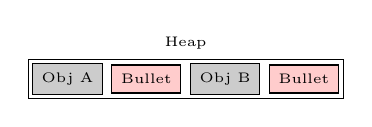
\begin{tikzpicture}[font=\tiny]
                \node[draw, minimum height=0.5cm, minimum width=4cm, label=above:Heap] {};
                \node[draw, fill=gray!40] at (-1.5,0) {Obj A};
                \node[draw, fill=red!20] at (-0.5,0) {Bullet};
                \node[draw, fill=gray!40] at (0.5,0) {Obj B};
                \node[draw, fill=red!20] at (1.5,0) {Bullet};
            \end{tikzpicture}
            }
            \textit{\small Terjadi fragmentasi memori.}
            
            \vspace{0.5cm}
            
            \textbf{Dengan Pool:}
            \resizebox{\textwidth}{!}{
            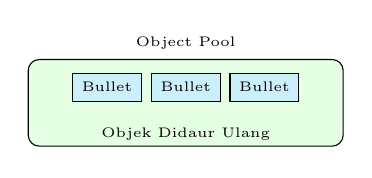
\begin{tikzpicture}[font=\tiny]
                \node[draw, fill=green!10, rounded corners, minimum height=1.1cm, minimum width=4cm, label=above:Object Pool] (pool) {};
                \node[draw, fill=cyan!20] at (-1, 0.2) {Bullet};
                \node[draw, fill=cyan!20] at (0, 0.2) {Bullet};
                \node[draw, fill=cyan!20] at (1, 0.2) {Bullet};
                \node at (0, -0.4) {Objek Didaur Ulang};
            \end{tikzpicture}
            }
            \textit{\small Memori stabil, tidak ada alokasi baru.}
        \end{column}
    \end{columns}
\end{spacing}
\end{frame}

\begin{frame}[t, fragile]
\frametitle{3: Mencegah Jeda GC}
\footnotesize
\begin{spacing}{0.85}
    Konsekuensi paling penting adalah berkurangnya beban kerja Garbage Collector secara drastis.

    \begin{columns}[T]
        \begin{column}{0.5\textwidth}
            \textbf{Penjelasan Solusi}
            
            Prinsipnya sederhana: \textbf{``Lebih sedikit sampah, lebih sedikit pekerjaan untuk tukang sampah.''}
            
            \begin{itemize}
                \item Karena objek tidak pernah benar-benar ``mati'' (hanya ``bebas'' di dalam pool), mereka tidak menjadi target GC.
                \item Dengan mengurangi jumlah objek yang harus dibersihkan, kita mengurangi frekuensi dan durasi jeda "Stop-the-World".
            \end{itemize}

            \begin{alertblock}{Hasil Akhir}
            Game berjalan jauh lebih mulus, dengan \textit{frame rate} yang stabil dan tanpa \textit{stutter} yang mengganggu. Ini adalah kunci untuk pengalaman bermain yang baik.
            \end{alertblock}
            
        \end{column}
        \begin{column}{0.5\textwidth}
            \textbf{Visualisasi Perbandingan Timeline}
            
            \textbf{Tanpa Pool:}
            \resizebox{0.9\textwidth}{!}{
            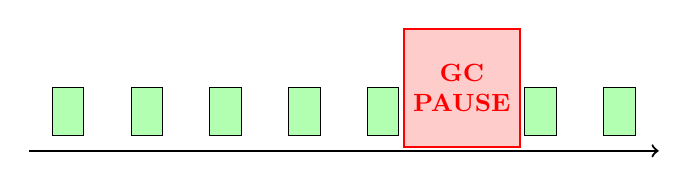
\begin{tikzpicture}[font=\small]
                \draw[->, thick] (0,0) -- (8,0);
                \foreach \x in {0.5, 1.5, ..., 4.5, 6.5, 7.5}
                    \draw[fill=green!30] (\x-0.2, 0.2) rectangle (\x+0.2, 0.8);
                \node[draw, red, thick, fill=red!20, minimum height=1.5cm, align=center]
                      at (5.5, 0.8) {\textbf{GC}\\\textbf{PAUSE}};
            \end{tikzpicture}
            }
            
            \vspace{0.5cm}
            
            \textbf{Dengan Pool:}
            \resizebox{0.9\textwidth}{!}{
            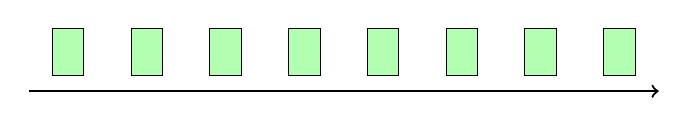
\begin{tikzpicture}[font=\small]
                \draw[->, thick] (0,0) -- (8,0);
                \foreach \x in {0.5, 1.5, ..., 7.5}
                    \draw[fill=green!30] (\x-0.2, 0.2) rectangle (\x+0.2, 0.8);
            \end{tikzpicture}
            }
            
        \end{column}
    \end{columns}
\end{spacing}
\end{frame}

\subsection{Kelemahan Object Pool Pattern}
\begin{frame}[t, fragile]
\frametitle{Reset State}
\vspace{-2mm}
\footnotesize
\begin{spacing}{0.85}
    Kekuatan utama Object Pool (performa) datang dengan tanggung jawab baru yang signifikan: manajemen state objek daur ulang.

    \begin{columns}[T]
        \begin{column}{0.35\textwidth}
            \textbf{Masalah: Objek ``Bekas Pakai''}
            
            Objek yang Anda \texttt{acquire()} dari pool bukanlah objek baru yang bersih. Ia adalah objek "bekas" yang mungkin masih membawa sisa-sisa state dari penggunaan sebelumnya.
            
            \begin{itemize}
                \item Anda \textbf{wajib} membuat metode \texttt{reset()} yang secara manual mengembalikan semua atribut objek ke keadaan awalnya.
                \item Lupa me-reset satu atribut saja bisa menyebabkan bug yang sangat sulit dilacak.
            \end{itemize}
            
            Ini menambah kompleksitas dan beban kerja bagi programmer.
            
        \end{column}
        \begin{column}{0.65\textwidth}
            \textbf{Contoh Bug Akibat Lupa Reset}
            
            Bayangkan sebuah peluru yang lupa di-reset status \texttt{isExploded}-nya.
            
            \begin{minted}[fontsize=\scriptsize, bgcolor=softred]{java}
public class Bullet {
    Vector2 position;
    Vector2 velocity;
    boolean isExploded = false;    
    // Metode ini LUPA me-reset isExploded!
    public void reset() {
        position.set(0, 0);
        velocity.set(0, 0);
    }
}
// Di dalam game loop...
// Peluru lama meledak dan dikembalikan ke pool
bullet.isExploded = true;
bulletPool.release(bullet);
// Peluru yang sama didaur ulang
Bullet newBullet = bulletPool.acquire();
// BUG! newBullet.isExploded masih true,
// sehingga ia langsung meledak saat muncul.
            \end{minted}
        \end{column}
    \end{columns}
\end{spacing}
\end{frame}

\begin{frame}[t, fragile]
\frametitle{Memory Leak}
\footnotesize
\begin{spacing}{0.85}
    Kelemahan lain yang berbahaya dari Object Pool adalah risiko kebocoran memori (memory leak) jika objek tidak dikelola dengan benar.

    \begin{columns}[T]
        \begin{column}{0.5\textwidth}
            \textbf{Masalah: Objek yang ``Hilang''}
            
            Pola ini bergantung sepenuhnya pada klien untuk mengembalikan objek dengan memanggil \texttt{release()}.
            
            \begin{itemize}
                \item Jika seorang programmer lupa memanggil \texttt{release()}, objek tersebut akan ``tersesat''.
                \item Ia tidak akan pernah kembali ke pool untuk didaur ulang.
                \item Parahnya, ia juga \textbf{tidak akan dibersihkan oleh Garbage Collector}, karena referensinya masih dipegang oleh klien (meskipun sudah tidak digunakan).
            \end{itemize}
            
            Seiring waktu, pool akan terus-menerus membuat objek baru untuk menggantikan yang hilang, menyebabkan memori membengkak.
        \end{column}
        \begin{column}{0.5\textwidth}
            \textbf{Contoh Kode yang Menyebabkan Leak}
            
            Di sini, peluru yang keluar layar dihapus dari daftar aktif, tetapi tidak dikembalikan ke pool.
            
            \begin{minted}[fontsize=\scriptsize, bgcolor=softred]{java}
// Di dalam game loop...
Iterator<Bullet> iter = activeBullets.iterator();
while (iter.hasNext()) {
    Bullet b = iter.next();
    b.update(delta);    
    if (b.isOffScreen()) {
        // BUG! Seharusnya ada panggilan:
        // bulletPool.release(b);
        
        // Objek dihapus dari daftar,
        // tapi tidak pernah kembali ke pool.
        // MEMORY LEAK!
        iter.remove();
    }
}
            \end{minted}
        \end{column}
    \end{columns}
\end{spacing}
\end{frame}

% ==================================================================
\section{Kesimpulan}
% ==================================================================
\SetSlideHeaderLevel{section}
\begin{frame}[t, fragile]
\frametitle{Analisis Pola Desain: Trade-offs}
\footnotesize
\begin{spacing}{0.85}
    Setiap pola desain adalah alat dengan kekuatan dan kelemahan. Kunci dari arsitektur yang baik adalah mengetahui kapan harus menggunakan alat yang tepat.

    \begin{columns}[T]
        \begin{column}{0.5\textwidth}
            \begin{block}{Factory Method}
                \textbf{Fokus: Fleksibilitas Desain}
                \begin{itemize}
                    \item[\CheckMark] \textbf{Pro:} Mendukung Prinsip Open/Closed. Menghilangkan ketergantungan pada kelas konkret, membuat sistem mudah diekstensi.
                    \item[\WarnSign] \textbf{Con:} Menambah jumlah kelas dalam proyek ("ledakan kelas"), yang bisa meningkatkan kompleksitas manajemen file.
                \end{itemize}
            \end{block}
        \end{column}
        \begin{column}{0.5\textwidth}
            \begin{block}{Object Pool}
                \textbf{Fokus: Efisiensi Performa}
                \begin{itemize}
                    \item[\CheckMark] \textbf{Pro:} Meningkatkan performa secara drastis dengan mengurangi alokasi memori dan jeda akibat Garbage Collection.
                    \item[\WarnSign] \textbf{Con:} Menambah kompleksitas. Kita harus mengelola siklus hidup objek, termasuk me-reset state-nya saat di-\texttt{release}.
                \end{itemize}
            \end{block}
        \end{column}
    \end{columns}

    \begin{alertblock}{Pesan Kunci}
    Tidak ada "peluru perak". Kita menukar satu jenis kompleksitas (misal: modifikasi file inti) dengan jenis kompleksitas lain (misal: jumlah file atau manajemen state).
    \end{alertblock}
\end{spacing}
\end{frame}

\begin{frame}[t, fragile]
\frametitle{Memilih Alat yang Tepat}
\vspace{-2mm}
\footnotesize
\justifying
\begin{spacing}{0.85}
\begin{columns}[T]
    \begin{column}{0.4\textwidth}
    Modul ini membawa kita dalam sebuah perjalanan untuk memecahkan dua masalah fundamental yang berbeda dalam pengembangan game.

    \begin{alertblock}{Pelajaran Utama}
    Pola desain bukanlah tujuan itu sendiri; mereka adalah \textbf{alat spesifik untuk memecahkan masalah spesifik}. Identifikasi masalah Anda terlebih dahulu, baru pilih alat yang tepat.
    \end{alertblock}

    \end{column}
    \begin{column}{0.6\textwidth}
    \centering
    \vspace{-6mm}
    \resizebox{0.5\textwidth}{!}{
    \begin{tikzpicture}[
        node distance=0.3cm and 1.5cm,
        block/.style={rectangle, draw, thick, fill=blue!10, text width=3.5cm,
                      minimum height=1.0cm, text centered, rounded corners},
        arrow/.style={draw, ->, >=Stealth, thick, color=blue!70!black}
    ]
        \node[block, fill=orange!10] (p1) {\textbf{1. Masalah Kekakuan} \\ \tiny Menambah variasi objek};
        \node[block, fill=cyan!10, below=of p1] (p2) {\textbf{2. Solusi Fleksibilitas} \\ \tiny Factory Method Pattern};
        \node[block, fill=orange!10, below=of p2] (p3) {\textbf{3. Masalah Performa} \\ \tiny Biaya `new' \& Jeda GC};
        \node[block, fill=cyan!10, below=of p3] (p4) {\textbf{4. Solusi Efisiensi} \\ \tiny Object Pool Pattern};
        \node[block, fill=green!10, below=of p4] (p5) {\textbf{5. Sinergi} \\ \tiny Pool + Factory};

        \draw[arrow] (p1) -- (p2); \draw[arrow] (p2) -- (p3);
        \draw[arrow] (p3) -- (p4); \draw[arrow] (p4) -- (p5);
    \end{tikzpicture}
    }
    \end{column}
\end{columns}
\end{spacing}
\end{frame}
